\begin{surferPage}[Barth-Sextik]{Die Barth-Sextik}
    Diese Fläche vom Grad $6$ --- daher Sextik --- hat Wolf Barth im Jahr 1996
    konstruiert.  

    Die Barth-Sextik hat insgesamt $65$ Singularitäten.
%    (wenn man die $15$ im Bild nicht sichtbaren, ``unendlich fernen'', mitzählt)%
    Dies ist die maximal mögliche Anzahl von Singularitäten auf einer Sextik,
    wie kurze Zeit später Jaffe und Ruberman zeigten --- Barths
    Weltrekord ist also unschlagbar!

    Barths Konstruktion war eine große Überraschung, da lange vermutet wurde,
    dass Flächen vom Grad $6$ nur $64$ Singularitäten haben können.

    Auffällig ist die Ikosaeder-Symmetrie der Konstruktion (das Bild zeigt den
    Ikosaeder und die Symmetrie-Ebenen): 
%    Die Abb.\ zeigt diesen platonischen Körper und seine Symmetrie - Ebenen: 
%    und diese Ebenen gemeinsam mit der Barth Sextik in einem Bild.     
    % 
    \begin{center}
      \vspace*{-0.1cm}
      \begin{tabular}{@{}c@{\ \ }c@{\,}c@{}}
        \begin{tabular}{@{}c}
          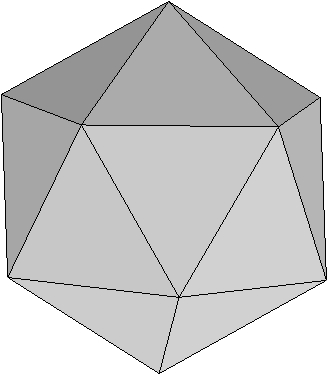
\includegraphics[width=1.4cm]{./../../common/images/icosah}
        \end{tabular}
        &
        \begin{tabular}{@{}c}
          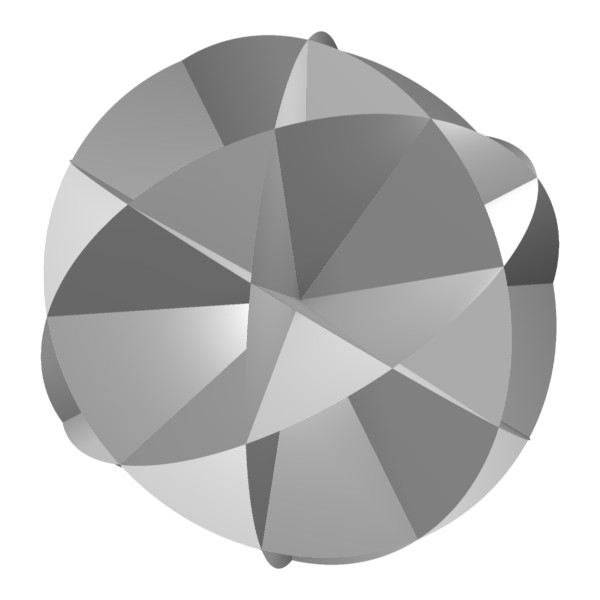
\includegraphics[width=1.4cm]{./../../common/images/barth_sextic_planes}
        \end{tabular}
        &
        \begin{tabular}{c@{}}
          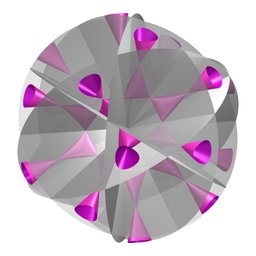
\includegraphics[width=1.4cm]{./../../common/images/barth_sextic_and_planes}
        \end{tabular}
      \end{tabular}
    \end{center}
    \vspace*{-0.1cm}
    Die Barth-Sextik erfüllt: $P_6 - \alpha K^2=0,$ wobei $P_6$ für die
    Symmetrie-Ebenen, $K=x^2+y^2+z^2-1$ für die Sphäre und
    $\alpha=\frac{1}{4}(2+\sqrt{5})$ steht. 
\end{surferPage}
